\documentclass[twoside]{book}

% Packages required by doxygen
\usepackage{fixltx2e}
\usepackage{calc}
\usepackage{doxygen}
\usepackage[export]{adjustbox} % also loads graphicx
\usepackage{graphicx}
\usepackage[utf8]{inputenc}
\usepackage{makeidx}
\usepackage{multicol}
\usepackage{multirow}
\PassOptionsToPackage{warn}{textcomp}
\usepackage{textcomp}
\usepackage[nointegrals]{wasysym}
\usepackage[table]{xcolor}

% Font selection
\usepackage[T1]{fontenc}
\usepackage[scaled=.90]{helvet}
\usepackage{courier}
\usepackage{amssymb}
\usepackage{sectsty}
\renewcommand{\familydefault}{\sfdefault}
\allsectionsfont{%
  \fontseries{bc}\selectfont%
  \color{darkgray}%
}
\renewcommand{\DoxyLabelFont}{%
  \fontseries{bc}\selectfont%
  \color{darkgray}%
}
\newcommand{\+}{\discretionary{\mbox{\scriptsize$\hookleftarrow$}}{}{}}

% Page & text layout
\usepackage{geometry}
\geometry{%
  a4paper,%
  top=2.5cm,%
  bottom=2.5cm,%
  left=2.5cm,%
  right=2.5cm%
}
\tolerance=750
\hfuzz=15pt
\hbadness=750
\setlength{\emergencystretch}{15pt}
\setlength{\parindent}{0cm}
\setlength{\parskip}{3ex plus 2ex minus 2ex}
\makeatletter
\renewcommand{\paragraph}{%
  \@startsection{paragraph}{4}{0ex}{-1.0ex}{1.0ex}{%
    \normalfont\normalsize\bfseries\SS@parafont%
  }%
}
\renewcommand{\subparagraph}{%
  \@startsection{subparagraph}{5}{0ex}{-1.0ex}{1.0ex}{%
    \normalfont\normalsize\bfseries\SS@subparafont%
  }%
}
\makeatother

% Headers & footers
\usepackage{fancyhdr}
\pagestyle{fancyplain}
\fancyhead[LE]{\fancyplain{}{\bfseries\thepage}}
\fancyhead[CE]{\fancyplain{}{}}
\fancyhead[RE]{\fancyplain{}{\bfseries\leftmark}}
\fancyhead[LO]{\fancyplain{}{\bfseries\rightmark}}
\fancyhead[CO]{\fancyplain{}{}}
\fancyhead[RO]{\fancyplain{}{\bfseries\thepage}}
\fancyfoot[LE]{\fancyplain{}{}}
\fancyfoot[CE]{\fancyplain{}{}}
\fancyfoot[RE]{\fancyplain{}{\bfseries\scriptsize Generated by Doxygen }}
\fancyfoot[LO]{\fancyplain{}{\bfseries\scriptsize Generated by Doxygen }}
\fancyfoot[CO]{\fancyplain{}{}}
\fancyfoot[RO]{\fancyplain{}{}}
\renewcommand{\footrulewidth}{0.4pt}
\renewcommand{\chaptermark}[1]{%
  \markboth{#1}{}%
}
\renewcommand{\sectionmark}[1]{%
  \markright{\thesection\ #1}%
}

% Indices & bibliography
\usepackage{natbib}
\usepackage[titles]{tocloft}
\setcounter{tocdepth}{3}
\setcounter{secnumdepth}{5}
\makeindex

% Hyperlinks (required, but should be loaded last)
\usepackage{ifpdf}
\ifpdf
  \usepackage[pdftex,pagebackref=true]{hyperref}
\else
  \usepackage[ps2pdf,pagebackref=true]{hyperref}
\fi
\hypersetup{%
  colorlinks=true,%
  linkcolor=blue,%
  citecolor=blue,%
  unicode%
}

% Custom commands
\newcommand{\clearemptydoublepage}{%
  \newpage{\pagestyle{empty}\cleardoublepage}%
}

\usepackage{caption}
\captionsetup{labelsep=space,justification=centering,font={bf},singlelinecheck=off,skip=4pt,position=top}

%===== C O N T E N T S =====

\begin{document}

% Titlepage & ToC
\hypersetup{pageanchor=false,
             bookmarksnumbered=true,
             pdfencoding=unicode
            }
\pagenumbering{alph}
\begin{titlepage}
\vspace*{7cm}
\begin{center}%
{\Large Mcts\+Core \\[1ex]\large 1.\+0 }\\
\vspace*{1cm}
{\large Generated by Doxygen 1.8.14}\\
\end{center}
\end{titlepage}
\clearemptydoublepage
\pagenumbering{roman}
\tableofcontents
\clearemptydoublepage
\pagenumbering{arabic}
\hypersetup{pageanchor=true}

%--- Begin generated contents ---
\chapter{Namespace Index}
\section{Packages}
Here are the packages with brief descriptions (if available)\+:\begin{DoxyCompactList}
\item\contentsline{section}{\mbox{\hyperlink{namespace_hus}{Hus}} }{\pageref{namespace_hus}}{}
\end{DoxyCompactList}

\chapter{Hierarchical Index}
\section{Class Hierarchy}
This inheritance list is sorted roughly, but not completely, alphabetically\+:\begin{DoxyCompactList}
\item \contentsline{section}{Game\+Tree\+Core.\+I\+Child\+Selection\+Service}{\pageref{interface_game_tree_core_1_1_i_child_selection_service}}{}
\begin{DoxyCompactList}
\item \contentsline{section}{Game\+Tree\+Core.\+Child\+Selection\+Service\+Alpha\+A\+M\+AF}{\pageref{class_game_tree_core_1_1_child_selection_service_alpha_a_m_a_f}}{}
\begin{DoxyCompactList}
\item \contentsline{section}{Game\+Tree\+Core.\+Child\+Selection\+Service\+A\+M\+AF}{\pageref{class_game_tree_core_1_1_child_selection_service_a_m_a_f}}{}
\item \contentsline{section}{Game\+Tree\+Core.\+Child\+Selection\+Service\+U\+CT}{\pageref{class_game_tree_core_1_1_child_selection_service_u_c_t}}{}
\end{DoxyCompactList}
\item \contentsline{section}{Game\+Tree\+Core.\+Child\+Selection\+Service\+R\+A\+VE}{\pageref{class_game_tree_core_1_1_child_selection_service_r_a_v_e}}{}
\item \contentsline{section}{Game\+Tree\+Core.\+Child\+Selection\+Service\+Silver\+Alpha\+A\+M\+AF}{\pageref{class_game_tree_core_1_1_child_selection_service_silver_alpha_a_m_a_f}}{}
\end{DoxyCompactList}
\item \contentsline{section}{Game\+Tree\+Core.\+I\+Final\+Child\+Selection\+Service}{\pageref{interface_game_tree_core_1_1_i_final_child_selection_service}}{}
\begin{DoxyCompactList}
\item \contentsline{section}{Game\+Tree\+Core.\+Final\+Child\+Selection\+Service\+M\+AX}{\pageref{class_game_tree_core_1_1_final_child_selection_service_m_a_x}}{}
\item \contentsline{section}{Game\+Tree\+Core.\+Final\+Child\+Selection\+Service\+R\+O\+B\+U\+ST}{\pageref{class_game_tree_core_1_1_final_child_selection_service_r_o_b_u_s_t}}{}
\item \contentsline{section}{Game\+Tree\+Core.\+Final\+Child\+Selection\+Service\+S\+E\+C\+U\+RE}{\pageref{class_game_tree_core_1_1_final_child_selection_service_s_e_c_u_r_e}}{}
\end{DoxyCompactList}
\item \contentsline{section}{Game\+Tree\+Core.\+I\+Game\+Tree\+Node}{\pageref{interface_game_tree_core_1_1_i_game_tree_node}}{}
\end{DoxyCompactList}

\chapter{Class Index}
\section{Class List}
Here are the classes, structs, unions and interfaces with brief descriptions\+:\begin{DoxyCompactList}
\item\contentsline{section}{\mbox{\hyperlink{class_game_tree_core_1_1_child_selection_service_alpha_a_m_a_f}{Game\+Tree\+Core.\+Child\+Selection\+Service\+Alpha\+A\+M\+AF}} \\*A child selection service based on the alpha A\+M\+AF algorithm. }{\pageref{class_game_tree_core_1_1_child_selection_service_alpha_a_m_a_f}}{}
\item\contentsline{section}{\mbox{\hyperlink{class_game_tree_core_1_1_child_selection_service_a_m_a_f}{Game\+Tree\+Core.\+Child\+Selection\+Service\+A\+M\+AF}} \\*A child selection service based on the A\+M\+AF algorithm. This is a special case of the alpha A\+M\+AF version (alpha = 1). }{\pageref{class_game_tree_core_1_1_child_selection_service_a_m_a_f}}{}
\item\contentsline{section}{\mbox{\hyperlink{class_game_tree_core_1_1_child_selection_service_r_a_v_e}{Game\+Tree\+Core.\+Child\+Selection\+Service\+R\+A\+VE}} \\*A child selection service based on the R\+A\+VE algorithm. }{\pageref{class_game_tree_core_1_1_child_selection_service_r_a_v_e}}{}
\item\contentsline{section}{\mbox{\hyperlink{class_game_tree_core_1_1_child_selection_service_silver_alpha_a_m_a_f}{Game\+Tree\+Core.\+Child\+Selection\+Service\+Silver\+Alpha\+A\+M\+AF}} \\*A child selection service based on the alpha A\+M\+AF algorithm from David Silver. }{\pageref{class_game_tree_core_1_1_child_selection_service_silver_alpha_a_m_a_f}}{}
\item\contentsline{section}{\mbox{\hyperlink{class_game_tree_core_1_1_child_selection_service_u_c_t}{Game\+Tree\+Core.\+Child\+Selection\+Service\+U\+CT}} \\*A child selection service based on the U\+CT algorithm. This is a special case of the alpha A\+M\+AF version (alpha = 0). }{\pageref{class_game_tree_core_1_1_child_selection_service_u_c_t}}{}
\item\contentsline{section}{\mbox{\hyperlink{class_game_tree_core_1_1_final_child_selection_service_m_a_x}{Game\+Tree\+Core.\+Final\+Child\+Selection\+Service\+M\+AX}} }{\pageref{class_game_tree_core_1_1_final_child_selection_service_m_a_x}}{}
\item\contentsline{section}{\mbox{\hyperlink{class_game_tree_core_1_1_final_child_selection_service_r_o_b_u_s_t}{Game\+Tree\+Core.\+Final\+Child\+Selection\+Service\+R\+O\+B\+U\+ST}} }{\pageref{class_game_tree_core_1_1_final_child_selection_service_r_o_b_u_s_t}}{}
\item\contentsline{section}{\mbox{\hyperlink{class_game_tree_core_1_1_final_child_selection_service_s_e_c_u_r_e}{Game\+Tree\+Core.\+Final\+Child\+Selection\+Service\+S\+E\+C\+U\+RE}} }{\pageref{class_game_tree_core_1_1_final_child_selection_service_s_e_c_u_r_e}}{}
\item\contentsline{section}{\mbox{\hyperlink{interface_game_tree_core_1_1_i_child_selection_service}{Game\+Tree\+Core.\+I\+Child\+Selection\+Service}} \\*Exposes a method to select a child node from a \mbox{\hyperlink{interface_game_tree_core_1_1_i_game_tree_node}{I\+Game\+Tree\+Node}}. }{\pageref{interface_game_tree_core_1_1_i_child_selection_service}}{}
\item\contentsline{section}{\mbox{\hyperlink{interface_game_tree_core_1_1_i_final_child_selection_service}{Game\+Tree\+Core.\+I\+Final\+Child\+Selection\+Service}} \\*Esposes a method to finally select a child node from a \mbox{\hyperlink{interface_game_tree_core_1_1_i_game_tree_node}{I\+Game\+Tree\+Node}}. }{\pageref{interface_game_tree_core_1_1_i_final_child_selection_service}}{}
\item\contentsline{section}{\mbox{\hyperlink{interface_game_tree_core_1_1_i_game_tree_node}{Game\+Tree\+Core.\+I\+Game\+Tree\+Node}} \\*Represents a node in a game tree. ~\newline
}{\pageref{interface_game_tree_core_1_1_i_game_tree_node}}{}
\end{DoxyCompactList}

\chapter{Namespace Documentation}
\hypertarget{namespace_mcts_core}{}\section{Mcts\+Core Namespace Reference}
\label{namespace_mcts_core}\index{Mcts\+Core@{Mcts\+Core}}
\subsection*{Classes}
\begin{DoxyCompactItemize}
\item 
class \mbox{\hyperlink{class_mcts_core_1_1_game_result}{Game\+Result}}
\begin{DoxyCompactList}\small\item\em Contains informations about the result of a game. \end{DoxyCompactList}\item 
interface \mbox{\hyperlink{interface_mcts_core_1_1_i_mctsable_game_state}{I\+Mctsable\+Game\+State}}
\begin{DoxyCompactList}\small\item\em Represents a game state for the mcts algorithm. \end{DoxyCompactList}\item 
interface \mbox{\hyperlink{interface_mcts_core_1_1_i_move}{I\+Move}}
\begin{DoxyCompactList}\small\item\em Represents a move of a game for the mcts algorithm. \end{DoxyCompactList}\item 
interface \mbox{\hyperlink{interface_mcts_core_1_1_i_non_deterministic_move}{I\+Non\+Deterministic\+Move}}
\begin{DoxyCompactList}\small\item\em Represents a non deterministic move of a game for the mcts algorithm. \end{DoxyCompactList}\item 
class \mbox{\hyperlink{class_mcts_core_1_1_mcts_algorithm}{Mcts\+Algorithm}}
\begin{DoxyCompactList}\small\item\em Provides static methods to calculate optimal moves using the mcts algorithm. \end{DoxyCompactList}\end{DoxyCompactItemize}

\chapter{Class Documentation}
\hypertarget{class_mcts_core_1_1_game_result}{}\section{Mcts\+Core.\+Game\+Result Class Reference}
\label{class_mcts_core_1_1_game_result}\index{Mcts\+Core.\+Game\+Result@{Mcts\+Core.\+Game\+Result}}


Contains informations about the result of a game.  


\subsection*{Public Member Functions}
\begin{DoxyCompactItemize}
\item 
\mbox{\hyperlink{class_mcts_core_1_1_game_result_a8c9838394b760c3e23498f1033be9727}{Game\+Result}} (int \mbox{\hyperlink{class_mcts_core_1_1_game_result_a77b59124aac0ba1f2cb5e0e131510cea}{winner}}, double \mbox{\hyperlink{class_mcts_core_1_1_game_result_a9620ecf5f08cc09f1d2ea5bf5568c3cc}{relative\+Victory\+Points}})
\begin{DoxyCompactList}\small\item\em Creates a new instance of the \mbox{\hyperlink{class_mcts_core_1_1_game_result}{Game\+Result}} class. \end{DoxyCompactList}\end{DoxyCompactItemize}
\subsection*{Properties}
\begin{DoxyCompactItemize}
\item 
static int \mbox{\hyperlink{class_mcts_core_1_1_game_result_acd7dea3def32dcf23531395d28688a4e}{no\+Winner}}\hspace{0.3cm}{\ttfamily  \mbox{[}get\mbox{]}}
\begin{DoxyCompactList}\small\item\em Represents a winner value in case of a draw. \end{DoxyCompactList}\item 
int \mbox{\hyperlink{class_mcts_core_1_1_game_result_a77b59124aac0ba1f2cb5e0e131510cea}{winner}}\hspace{0.3cm}{\ttfamily  \mbox{[}get\mbox{]}}
\begin{DoxyCompactList}\small\item\em Gets the winner corresponding to this game result. \end{DoxyCompactList}\item 
double \mbox{\hyperlink{class_mcts_core_1_1_game_result_a9620ecf5f08cc09f1d2ea5bf5568c3cc}{relative\+Victory\+Points}}\hspace{0.3cm}{\ttfamily  \mbox{[}get\mbox{]}}
\begin{DoxyCompactList}\small\item\em Gets the achieved relative victory points corresponding to this game result. \end{DoxyCompactList}\end{DoxyCompactItemize}


\subsection{Detailed Description}
Contains informations about the result of a game. 



Definition at line 7 of file Game\+Result.\+cs.



\subsection{Constructor \& Destructor Documentation}
\mbox{\Hypertarget{class_mcts_core_1_1_game_result_a8c9838394b760c3e23498f1033be9727}\label{class_mcts_core_1_1_game_result_a8c9838394b760c3e23498f1033be9727}} 
\index{Mcts\+Core\+::\+Game\+Result@{Mcts\+Core\+::\+Game\+Result}!Game\+Result@{Game\+Result}}
\index{Game\+Result@{Game\+Result}!Mcts\+Core\+::\+Game\+Result@{Mcts\+Core\+::\+Game\+Result}}
\subsubsection{\texorpdfstring{Game\+Result()}{GameResult()}}
{\footnotesize\ttfamily Mcts\+Core.\+Game\+Result.\+Game\+Result (\begin{DoxyParamCaption}\item[{int}]{winner,  }\item[{double}]{relative\+Victory\+Points }\end{DoxyParamCaption})}



Creates a new instance of the \mbox{\hyperlink{class_mcts_core_1_1_game_result}{Game\+Result}} class. 


\begin{DoxyParams}{Parameters}
{\em winner} & The player who has won the game. I case of a draw use no\+Winner.\\
\hline
{\em relative\+Victory\+Points} & The ratio of achieved victory points to maximal victory points.\\
\hline
\end{DoxyParams}

\begin{DoxyExceptions}{Exceptions}
{\em Argument\+Exception} & Is thrown, if the given ratio is not in \mbox{[}0,1\mbox{]}.\\
\hline
\end{DoxyExceptions}


Definition at line 22 of file Game\+Result.\+cs.



\subsection{Property Documentation}
\mbox{\Hypertarget{class_mcts_core_1_1_game_result_acd7dea3def32dcf23531395d28688a4e}\label{class_mcts_core_1_1_game_result_acd7dea3def32dcf23531395d28688a4e}} 
\index{Mcts\+Core\+::\+Game\+Result@{Mcts\+Core\+::\+Game\+Result}!no\+Winner@{no\+Winner}}
\index{no\+Winner@{no\+Winner}!Mcts\+Core\+::\+Game\+Result@{Mcts\+Core\+::\+Game\+Result}}
\subsubsection{\texorpdfstring{no\+Winner}{noWinner}}
{\footnotesize\ttfamily int Mcts\+Core.\+Game\+Result.\+no\+Winner\hspace{0.3cm}{\ttfamily [static]}, {\ttfamily [get]}}



Represents a winner value in case of a draw. 



Definition at line 14 of file Game\+Result.\+cs.

\mbox{\Hypertarget{class_mcts_core_1_1_game_result_a9620ecf5f08cc09f1d2ea5bf5568c3cc}\label{class_mcts_core_1_1_game_result_a9620ecf5f08cc09f1d2ea5bf5568c3cc}} 
\index{Mcts\+Core\+::\+Game\+Result@{Mcts\+Core\+::\+Game\+Result}!relative\+Victory\+Points@{relative\+Victory\+Points}}
\index{relative\+Victory\+Points@{relative\+Victory\+Points}!Mcts\+Core\+::\+Game\+Result@{Mcts\+Core\+::\+Game\+Result}}
\subsubsection{\texorpdfstring{relative\+Victory\+Points}{relativeVictoryPoints}}
{\footnotesize\ttfamily double Mcts\+Core.\+Game\+Result.\+relative\+Victory\+Points\hspace{0.3cm}{\ttfamily [get]}}



Gets the achieved relative victory points corresponding to this game result. 



Definition at line 37 of file Game\+Result.\+cs.

\mbox{\Hypertarget{class_mcts_core_1_1_game_result_a77b59124aac0ba1f2cb5e0e131510cea}\label{class_mcts_core_1_1_game_result_a77b59124aac0ba1f2cb5e0e131510cea}} 
\index{Mcts\+Core\+::\+Game\+Result@{Mcts\+Core\+::\+Game\+Result}!winner@{winner}}
\index{winner@{winner}!Mcts\+Core\+::\+Game\+Result@{Mcts\+Core\+::\+Game\+Result}}
\subsubsection{\texorpdfstring{winner}{winner}}
{\footnotesize\ttfamily int Mcts\+Core.\+Game\+Result.\+winner\hspace{0.3cm}{\ttfamily [get]}}



Gets the winner corresponding to this game result. 



Definition at line 32 of file Game\+Result.\+cs.


\hypertarget{interface_mcts_core_1_1_i_mctsable_game_state}{}\section{Mcts\+Core.\+I\+Mctsable\+Game\+State Interface Reference}
\label{interface_mcts_core_1_1_i_mctsable_game_state}\index{Mcts\+Core.\+I\+Mctsable\+Game\+State@{Mcts\+Core.\+I\+Mctsable\+Game\+State}}


Represents a game state for the mcts algorithm.  


\subsection*{Public Member Functions}
\begin{DoxyCompactItemize}
\item 
\mbox{\Hypertarget{interface_mcts_core_1_1_i_mctsable_game_state_a56d2cadef7e60b1c334b9c10c20b6d18}\label{interface_mcts_core_1_1_i_mctsable_game_state_a56d2cadef7e60b1c334b9c10c20b6d18}} 
void {\bfseries make\+Move} (\mbox{\hyperlink{interface_mcts_core_1_1_i_move}{I\+Move}} move)
\item 
\mbox{\Hypertarget{interface_mcts_core_1_1_i_mctsable_game_state_aec80aafd8592e5f686b3c6ea2b4e1190}\label{interface_mcts_core_1_1_i_mctsable_game_state_aec80aafd8592e5f686b3c6ea2b4e1190}} 
bool {\bfseries is\+Game\+Over} ()
\item 
\mbox{\Hypertarget{interface_mcts_core_1_1_i_mctsable_game_state_a0a8f5d003e52adb2af90878067f8838f}\label{interface_mcts_core_1_1_i_mctsable_game_state_a0a8f5d003e52adb2af90878067f8838f}} 
\mbox{\hyperlink{interface_mcts_core_1_1_i_mctsable_game_state}{I\+Mctsable\+Game\+State}} {\bfseries duplicate} ()
\item 
\mbox{\Hypertarget{interface_mcts_core_1_1_i_mctsable_game_state_aaec4b1d3947fc0a15f9cee09d8916425}\label{interface_mcts_core_1_1_i_mctsable_game_state_aaec4b1d3947fc0a15f9cee09d8916425}} 
List$<$ \mbox{\hyperlink{interface_mcts_core_1_1_i_move}{I\+Move}} $>$ {\bfseries get\+Possible\+Moves} ()
\item 
\mbox{\Hypertarget{interface_mcts_core_1_1_i_mctsable_game_state_ac3466b8f70e507775f3f5a946ca4fbc5}\label{interface_mcts_core_1_1_i_mctsable_game_state_ac3466b8f70e507775f3f5a946ca4fbc5}} 
\mbox{\hyperlink{class_mcts_core_1_1_game_result}{Game\+Result}} {\bfseries get\+Result\+Of\+The\+Game} ()
\end{DoxyCompactItemize}
\subsection*{Properties}
\begin{DoxyCompactItemize}
\item 
\mbox{\Hypertarget{interface_mcts_core_1_1_i_mctsable_game_state_af6f55eec4b0c1b18ee5f19951d605964}\label{interface_mcts_core_1_1_i_mctsable_game_state_af6f55eec4b0c1b18ee5f19951d605964}} 
int {\bfseries phasing\+Player}\hspace{0.3cm}{\ttfamily  \mbox{[}get\mbox{]}}
\end{DoxyCompactItemize}


\subsection{Detailed Description}
Represents a game state for the mcts algorithm. 



Definition at line 7 of file I\+Mctsable\+Game\+State.\+cs.


\hypertarget{interface_mcts_core_1_1_i_move}{}\section{Mcts\+Core.\+I\+Move Interface Reference}
\label{interface_mcts_core_1_1_i_move}\index{Mcts\+Core.\+I\+Move@{Mcts\+Core.\+I\+Move}}


Represents a move of a game for the mcts algorithm.  


Inheritance diagram for Mcts\+Core.\+I\+Move\+:\begin{figure}[H]
\begin{center}
\leavevmode
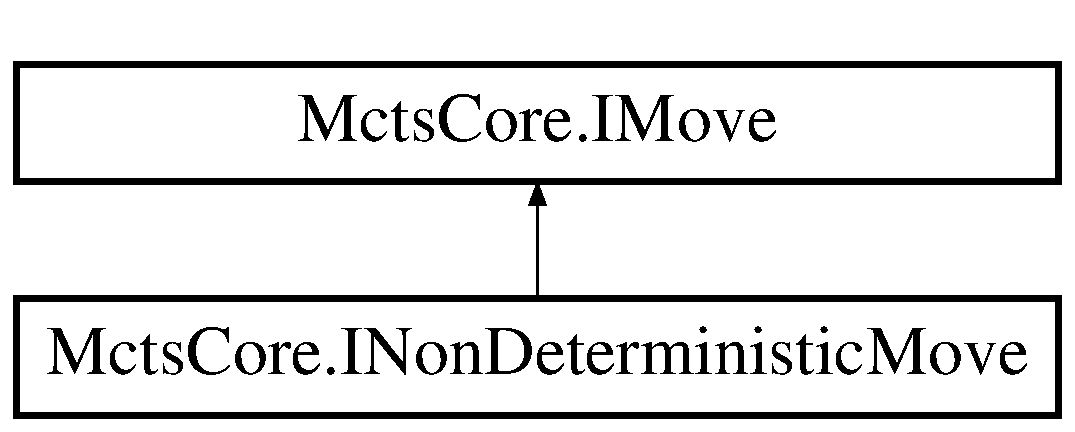
\includegraphics[height=2.000000cm]{interface_mcts_core_1_1_i_move}
\end{center}
\end{figure}
\subsection*{Public Member Functions}
\begin{DoxyCompactItemize}
\item 
\mbox{\Hypertarget{interface_mcts_core_1_1_i_move_a50974d40230b5da8a75bee6f4c9efda2}\label{interface_mcts_core_1_1_i_move_a50974d40230b5da8a75bee6f4c9efda2}} 
bool {\bfseries is\+Equal\+To} (\mbox{\hyperlink{interface_mcts_core_1_1_i_move}{I\+Move}} move)
\end{DoxyCompactItemize}
\subsection*{Properties}
\begin{DoxyCompactItemize}
\item 
\mbox{\Hypertarget{interface_mcts_core_1_1_i_move_aad81f4a0263011457c6c78a3886171cd}\label{interface_mcts_core_1_1_i_move_aad81f4a0263011457c6c78a3886171cd}} 
int {\bfseries next\+Player}\hspace{0.3cm}{\ttfamily  \mbox{[}get\mbox{]}}
\item 
\mbox{\Hypertarget{interface_mcts_core_1_1_i_move_a06f1d55f83bd7652cc3093c875f74e4c}\label{interface_mcts_core_1_1_i_move_a06f1d55f83bd7652cc3093c875f74e4c}} 
int {\bfseries player\+Who\+Does\+The\+Move}\hspace{0.3cm}{\ttfamily  \mbox{[}get\mbox{]}}
\end{DoxyCompactItemize}


\subsection{Detailed Description}
Represents a move of a game for the mcts algorithm. 



Definition at line 5 of file I\+Move.\+cs.


\hypertarget{interface_mcts_core_1_1_i_non_deterministic_move}{}\section{Mcts\+Core.\+I\+Non\+Deterministic\+Move Interface Reference}
\label{interface_mcts_core_1_1_i_non_deterministic_move}\index{Mcts\+Core.\+I\+Non\+Deterministic\+Move@{Mcts\+Core.\+I\+Non\+Deterministic\+Move}}


Represents a non deterministic move of a game for the mcts algorithm.  


Inheritance diagram for Mcts\+Core.\+I\+Non\+Deterministic\+Move\+:\begin{figure}[H]
\begin{center}
\leavevmode
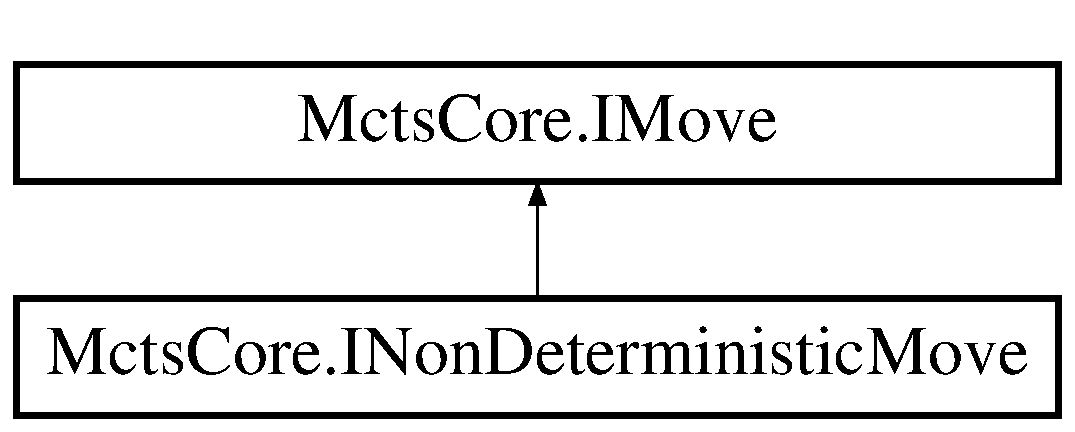
\includegraphics[height=2.000000cm]{interface_mcts_core_1_1_i_non_deterministic_move}
\end{center}
\end{figure}
\subsection*{Public Member Functions}
\begin{DoxyCompactItemize}
\item 
\mbox{\Hypertarget{interface_mcts_core_1_1_i_non_deterministic_move_a321f15d3c84bb9f79eb17cbf3ff7af79}\label{interface_mcts_core_1_1_i_non_deterministic_move_a321f15d3c84bb9f79eb17cbf3ff7af79}} 
Read\+Only\+Collection$<$ double $>$ {\bfseries get\+Child\+Distribution} ()
\end{DoxyCompactItemize}
\subsection*{Additional Inherited Members}


\subsection{Detailed Description}
Represents a non deterministic move of a game for the mcts algorithm. 



Definition at line 7 of file I\+Non\+Deterministic\+Move.\+cs.


\hypertarget{class_mcts_core_1_1_mcts_algorithm}{}\section{Mcts\+Core.\+Mcts\+Algorithm Class Reference}
\label{class_mcts_core_1_1_mcts_algorithm}\index{Mcts\+Core.\+Mcts\+Algorithm@{Mcts\+Core.\+Mcts\+Algorithm}}


Provides static methods to calculate optimal moves using the mcts algorithm.  


\subsection*{Static Public Member Functions}
\begin{DoxyCompactItemize}
\item 
static \mbox{\hyperlink{interface_mcts_core_1_1_i_move}{I\+Move}} \mbox{\hyperlink{class_mcts_core_1_1_mcts_algorithm_a9c380699425b42217d10608b797b69f5}{calculate\+Optimal\+Move\+With\+Given\+Iterations}} (\mbox{\hyperlink{interface_mcts_core_1_1_i_mctsable_game_state}{I\+Mctsable\+Game\+State}} inital\+Game\+State, int \mbox{\hyperlink{class_mcts_core_1_1_mcts_algorithm_ae871efb153533b29759ac01fbb2845ab}{iterations}}, I\+Child\+Selection\+Service child\+Selection\+Service, I\+Final\+Child\+Selection\+Service final\+Child\+Selection\+Service)
\begin{DoxyCompactList}\small\item\em Calculates the best move depending on the given game state and the given constraints. \end{DoxyCompactList}\item 
static \mbox{\hyperlink{interface_mcts_core_1_1_i_move}{I\+Move}} \mbox{\hyperlink{class_mcts_core_1_1_mcts_algorithm_a3ba9b28883c962188035e2f16c1c43a0}{calculate\+Optimal\+Move\+In\+Given\+Time}} (\mbox{\hyperlink{interface_mcts_core_1_1_i_mctsable_game_state}{I\+Mctsable\+Game\+State}} inital\+Game\+State, int time, I\+Child\+Selection\+Service child\+Selection\+Service, I\+Final\+Child\+Selection\+Service final\+Child\+Selection\+Service)
\begin{DoxyCompactList}\small\item\em Calculates the best move depending on the given game state and the given constraints. \end{DoxyCompactList}\end{DoxyCompactItemize}
\subsection*{Properties}
\begin{DoxyCompactItemize}
\item 
static int \mbox{\hyperlink{class_mcts_core_1_1_mcts_algorithm_ae871efb153533b29759ac01fbb2845ab}{iterations}}\hspace{0.3cm}{\ttfamily  \mbox{[}get\mbox{]}}
\begin{DoxyCompactList}\small\item\em Gets the number of done iterations until the final move was selected. \end{DoxyCompactList}\end{DoxyCompactItemize}


\subsection{Detailed Description}
Provides static methods to calculate optimal moves using the mcts algorithm. 



Definition at line 11 of file Mcts\+Algorithm.\+cs.



\subsection{Member Function Documentation}
\mbox{\Hypertarget{class_mcts_core_1_1_mcts_algorithm_a3ba9b28883c962188035e2f16c1c43a0}\label{class_mcts_core_1_1_mcts_algorithm_a3ba9b28883c962188035e2f16c1c43a0}} 
\index{Mcts\+Core\+::\+Mcts\+Algorithm@{Mcts\+Core\+::\+Mcts\+Algorithm}!calculate\+Optimal\+Move\+In\+Given\+Time@{calculate\+Optimal\+Move\+In\+Given\+Time}}
\index{calculate\+Optimal\+Move\+In\+Given\+Time@{calculate\+Optimal\+Move\+In\+Given\+Time}!Mcts\+Core\+::\+Mcts\+Algorithm@{Mcts\+Core\+::\+Mcts\+Algorithm}}
\subsubsection{\texorpdfstring{calculate\+Optimal\+Move\+In\+Given\+Time()}{calculateOptimalMoveInGivenTime()}}
{\footnotesize\ttfamily static \mbox{\hyperlink{interface_mcts_core_1_1_i_move}{I\+Move}} Mcts\+Core.\+Mcts\+Algorithm.\+calculate\+Optimal\+Move\+In\+Given\+Time (\begin{DoxyParamCaption}\item[{\mbox{\hyperlink{interface_mcts_core_1_1_i_mctsable_game_state}{I\+Mctsable\+Game\+State}}}]{inital\+Game\+State,  }\item[{int}]{time,  }\item[{I\+Child\+Selection\+Service}]{child\+Selection\+Service,  }\item[{I\+Final\+Child\+Selection\+Service}]{final\+Child\+Selection\+Service }\end{DoxyParamCaption})\hspace{0.3cm}{\ttfamily [static]}}



Calculates the best move depending on the given game state and the given constraints. 


\begin{DoxyParams}{Parameters}
{\em inital\+Game\+State} & A game state.\\
\hline
{\em time} & A time in milliseconds until a move is finally selected.\\
\hline
{\em child\+Selection\+Service} & A child selection service which is used during the mcts algorithm.\\
\hline
{\em final\+Child\+Selection\+Service} & A child selection service to finally select a child.\\
\hline
\end{DoxyParams}

\begin{DoxyExceptions}{Exceptions}
{\em Argument\+Null\+Exception} & Is thrown, if at least one of the given parameters is null.\\
\hline
{\em Argument\+Exception} & Is thrown, if the given game state is a terminal game state.\\
\hline
{\em Argument\+Exception} & Is thrown, if the given number of milliseconds is lower or equal than zero.\\
\hline
\end{DoxyExceptions}


Definition at line 111 of file Mcts\+Algorithm.\+cs.

\mbox{\Hypertarget{class_mcts_core_1_1_mcts_algorithm_a9c380699425b42217d10608b797b69f5}\label{class_mcts_core_1_1_mcts_algorithm_a9c380699425b42217d10608b797b69f5}} 
\index{Mcts\+Core\+::\+Mcts\+Algorithm@{Mcts\+Core\+::\+Mcts\+Algorithm}!calculate\+Optimal\+Move\+With\+Given\+Iterations@{calculate\+Optimal\+Move\+With\+Given\+Iterations}}
\index{calculate\+Optimal\+Move\+With\+Given\+Iterations@{calculate\+Optimal\+Move\+With\+Given\+Iterations}!Mcts\+Core\+::\+Mcts\+Algorithm@{Mcts\+Core\+::\+Mcts\+Algorithm}}
\subsubsection{\texorpdfstring{calculate\+Optimal\+Move\+With\+Given\+Iterations()}{calculateOptimalMoveWithGivenIterations()}}
{\footnotesize\ttfamily static \mbox{\hyperlink{interface_mcts_core_1_1_i_move}{I\+Move}} Mcts\+Core.\+Mcts\+Algorithm.\+calculate\+Optimal\+Move\+With\+Given\+Iterations (\begin{DoxyParamCaption}\item[{\mbox{\hyperlink{interface_mcts_core_1_1_i_mctsable_game_state}{I\+Mctsable\+Game\+State}}}]{inital\+Game\+State,  }\item[{int}]{iterations,  }\item[{I\+Child\+Selection\+Service}]{child\+Selection\+Service,  }\item[{I\+Final\+Child\+Selection\+Service}]{final\+Child\+Selection\+Service }\end{DoxyParamCaption})\hspace{0.3cm}{\ttfamily [static]}}



Calculates the best move depending on the given game state and the given constraints. 


\begin{DoxyParams}{Parameters}
{\em inital\+Game\+State} & A game state.\\
\hline
{\em iterations} & A number of iterations until a move is finally selected.\\
\hline
{\em child\+Selection\+Service} & A child selection service which is used during the mcts algorithm.\\
\hline
{\em final\+Child\+Selection\+Service} & A child selection service to finally select a child.\\
\hline
\end{DoxyParams}

\begin{DoxyExceptions}{Exceptions}
{\em Argument\+Null\+Exception} & Is thrown, if at least one of the given parameters is null.\\
\hline
{\em Argument\+Exception} & Is thrown, if the given game state is a terminal game state.\\
\hline
{\em Argument\+Exception} & Is thrown, if the number given iterations is lower or equal than zero.\\
\hline
\end{DoxyExceptions}


Definition at line 74 of file Mcts\+Algorithm.\+cs.



\subsection{Property Documentation}
\mbox{\Hypertarget{class_mcts_core_1_1_mcts_algorithm_ae871efb153533b29759ac01fbb2845ab}\label{class_mcts_core_1_1_mcts_algorithm_ae871efb153533b29759ac01fbb2845ab}} 
\index{Mcts\+Core\+::\+Mcts\+Algorithm@{Mcts\+Core\+::\+Mcts\+Algorithm}!iterations@{iterations}}
\index{iterations@{iterations}!Mcts\+Core\+::\+Mcts\+Algorithm@{Mcts\+Core\+::\+Mcts\+Algorithm}}
\subsubsection{\texorpdfstring{iterations}{iterations}}
{\footnotesize\ttfamily int Mcts\+Core.\+Mcts\+Algorithm.\+iterations\hspace{0.3cm}{\ttfamily [static]}, {\ttfamily [get]}}



Gets the number of done iterations until the final move was selected. 



Definition at line 62 of file Mcts\+Algorithm.\+cs.


%--- End generated contents ---

% Index
\backmatter
\newpage
\phantomsection
\clearemptydoublepage
\addcontentsline{toc}{chapter}{Index}
\printindex

\end{document}
